% Conceptual explanation of sparse joint cells and candidate-pool expansion.
% Included from main_edit_rev2.tex; requires TikZ and the positioning library.

\subsection{Sparse Joint Cells and Candidate-Pool Expansion}
\label{sec:missing_cells_framework}

Marginal controls can require combinations that are absent, or too rare, in
the observed microdata. This is a support problem rather than evidence that
the corresponding census cell is invalid. If the fitting pool contains no
candidate for a required joint cell, reweighting alone cannot populate that
cell: IPU or raking can change weights on existing records but cannot create a
new record with an unseen combination. Candidate-pool expansion addresses this
limitation before the final marginal-fitting step. The GAN and CP routes are
alternative mechanisms for proposing additional candidates; the SA/IPU stage
then selects or weights candidates against the reconciled controls.

\begin{figure}[htbp]
\centering
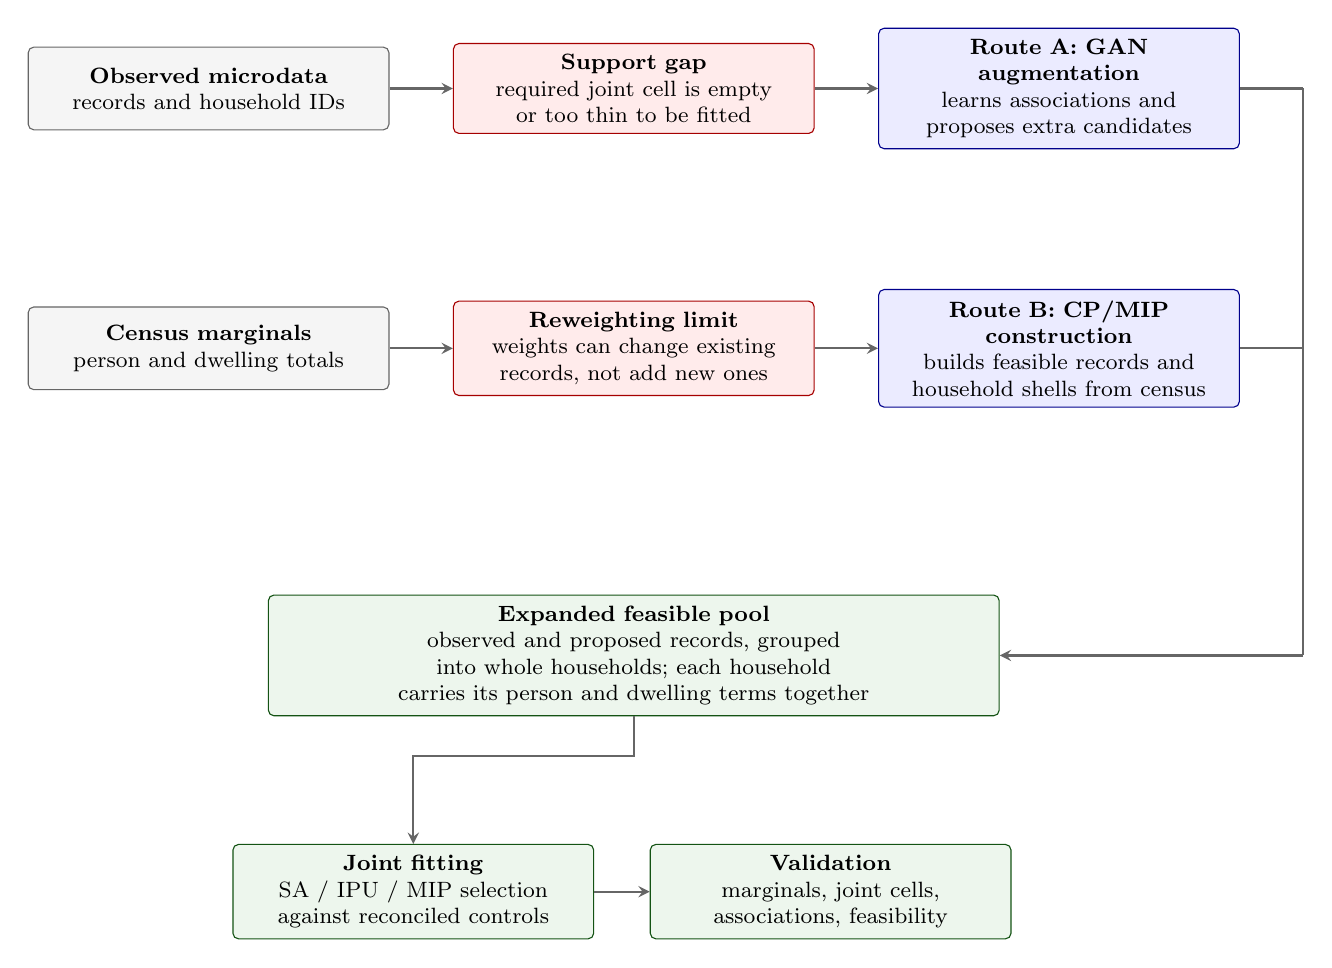
\begin{tikzpicture}[
  >=stealth,
  every node/.style={font=\footnotesize},
  box/.style={draw, rounded corners=2pt, align=center, inner sep=4pt,
              text width=4.3cm, minimum height=1.05cm},
  data/.style={box, draw=black!60, fill=gray!8},
  problem/.style={box, draw=red!65!black, fill=red!8},
  method/.style={box, draw=blue!55!black, fill=blue!8},
  result/.style={box, draw=ForestGreen!60!black, fill=ForestGreen!8},
  flow/.style={->, line width=0.8pt, draw=black!60},
  bus/.style={line width=0.8pt, draw=black!60},
]

%% , - row 1: what is observed, and one expansion route , , , , , , -
\node[data]    (micro)   at (0.0,0)    {\textbf{Observed microdata}\\
                                        records and household IDs};
\node[problem] (support) at (5.4,0)    {\textbf{Support gap}\\
                                        required joint cell is empty\\
                                        or too thin to be fitted};
\node[method]  (gan)     at (10.8,0)   {\textbf{Route A: GAN}\\
                                        \textbf{augmentation}\\
                                        learns associations and\\
                                        proposes extra candidates};

%% , - row 2: what is targeted, and the other route , , , , , , , --
\node[data]    (margins) at (0.0,-3.3) {\textbf{Census marginals}\\
                                        person and dwelling totals};
\node[problem] (weights) at (5.4,-3.3) {\textbf{Reweighting limit}\\
                                        weights can change existing\\
                                        records, not add new ones};
\node[method]  (cp)      at (10.8,-3.3){\textbf{Route B: CP/MIP}\\
                                        \textbf{construction}\\
                                        builds feasible records and\\
                                        household shells from census};

%% , - merged pool , , , , , , , , , , , , , , , , , , --
\node[result, text width=9.0cm] (pool) at (5.4,-7.2)
  {\textbf{Expanded feasible pool}\\
   observed and proposed records, grouped\\
   into whole households; each household\\
   carries its person and dwelling terms together};

%% , - fitting and validation , , , , , , , , , , , , , , --
\node[result] (fit) at (2.6,-10.2)
  {\textbf{Joint fitting}\\ SA / IPU / MIP selection\\ against reconciled controls};
\node[result] (validate) at (7.9,-10.2)
  {\textbf{Validation}\\ marginals, joint cells,\\ associations, feasibility};

%% , - edges , , , , , , , , , , , , , , , , , , , , --
\draw[flow] (micro) -- (support);
\draw[flow] (support) -- (gan);
\draw[flow] (margins) -- (weights);
\draw[flow] (weights) -- (cp);

% Both routes feed a single vertical bus clear of the boxes on the right,
% which enters the pool once; this keeps the long arrows off the row-2 nodes.
\draw[bus] (gan.east) -- (13.9,0);
\draw[bus] (cp.east) -- (13.9,-3.3);
\draw[bus] (13.9,0) -- (13.9,-7.2);
\draw[flow] (13.9,-7.2) -- (pool.east);

\draw[flow] (pool.south) -- ++(0,-0.5) -| (fit.north);
\draw[flow] (fit.east) -- (validate.west);

\end{tikzpicture}%
\caption{Conceptual role of candidate-pool expansion. A missing joint cell
cannot be repaired by reweighting alone because no observed record carries
the required combination. GAN augmentation (route A) and CP/MIP construction
(route B) provide different mechanisms for proposing feasible candidates, and
both enter the same pool; the final fitting stage must still reconcile person
and dwelling universes and validate both marginal and joint structure.
Proposed records are admitted as complete households rather than as
free-floating persons, so pool expansion and household construction are
coupled: whichever route supplies a record also fixes the dwelling terms its
housemates must share.}
\label{fig:missing-cells-framework}
\end{figure}

\paragraph{Interpretation.}
The figure does not imply that every unseen combination is realistic. A
candidate is retained only when it satisfies the applicable structural rules,
household-integrity checks, and downstream marginal/joint validation. Novelty
therefore indicates absence from the observed microdata, not empirical proof
that a combination is absent from the population; Appendix~\ref{sec:pool_expansion_audit} reports the pool-expansion audit: how many zero cells the mechanism fills, with how many records, and which cells it cannot source.

